% Created 2023-05-19 Fri 15:59
% Intended LaTeX compiler: xelatex
\documentclass[aspectratio=1610,xcolor={dvipsnames},hyperref={colorlinks,unicode,linkcolor=violet,anchorcolor=BlueViolet,citecolor=YellowOrange,filecolor=black,urlcolor=Aquamarine}]{beamer}
\usepackage{graphicx}
\usepackage{grffile}
\usepackage{longtable}
\usepackage{booktabs}
\usepackage{wrapfig}
\usepackage{rotating}
\usepackage[normalem]{ulem}
\usepackage{amsmath}
\usepackage{textcomp}
\usepackage{amssymb}
\usepackage{capt-of}
\usepackage{nicefrac}
\usepackage[dvipsnames]{xcolor}
\usepackage[colorlinks,unicode,linkcolor=violet,anchorcolor=BlueViolet,citecolor=YellowOrange,filecolor=black,urlcolor=Aquamarine]{hyperref}
\AtBeginSubsection[]{\begin{frame}<beamer>\frametitle{Section}\tableofcontents[currentsection,currentsubsection]\end{frame}}
\synctex=1
\usepackage{etoolbox}
\useoutertheme{infolines}
\setbeamertemplate{frametitle}{%
\usebeamerfont{frametitle}\insertframetitle\strut%
\vskip-0\baselineskip%
\leaders\vrule width .95\paperwidth\vskip1pt%
\vskip0pt%
\nointerlineskip%
}

%% T for footer
\setbeamercolor{footlinecolor}{fg=cyan,bg=green}
\setbeamercolor{author in head/foot}{fg=blue}
\setbeamertemplate{footline}{%
\leavevmode%
\hbox{%
\begin{beamercolorbox}[wd=.26\paperwidth,ht=2.25ex,dp=1ex,left]{author in head/foot}%
\hspace*{2ex}\usebeamerfont{author in head/foot} Dept. CSE, UT Arlington
\end{beamercolorbox}%
\begin{beamercolorbox}[wd=.50\paperwidth,ht=2.25ex,dp=1ex,center]{author in head/foot}%
\usebeamerfont{title in head/foot}Scalable Modeling \& Imaging \& Learning Lab (SMILE)
\end{beamercolorbox}%
\begin{beamercolorbox}[wd=.24\paperwidth,ht=2.25ex,dp=1ex,right]{date in head/foot}%
\usebeamerfont{date in head/foot}
\insertshortdate{}\hspace*{1em}  % date
\insertframenumber/\inserttotalframenumber\hspace*{2ex}
\end{beamercolorbox}}%
\vskip0pt%
}
\setbeamerfont{footnote}{size=\tiny}
\usepackage{minted}
\setbeamerfont{caption}{size=\scriptsize}
\usetheme{default}
\usefonttheme{serif}
\useinnertheme{circles}
\author{Nasy}
\date{May 19, 2023}
\title{LLM Fine-tuning}
\hypersetup{
 pdfauthor={Nasy},
 pdftitle={LLM Fine-tuning},
 pdfkeywords={},
 pdfsubject={},
 pdfcreator={Emacs 29.0.50 (Org mode 9.5.5)}, 
 pdflang={English}}
\usepackage{biblatex}
\addbibresource{/Users/Nasy/.emacs.d/萚兮/時/refs/ref.bib}
\begin{document}

\maketitle
\begin{frame}{Outline}
\setcounter{tocdepth}{1}
\tableofcontents
\end{frame}

\setcounter{tocdepth}{2}

\section{Introduction}
\label{sec:org6d902f1}

\begin{frame}[label={sec:orgdce5aba}]{Introduction}
\begin{itemize}
\item Which model to choice?
\item How to fine-tune?
\item Examples
\end{itemize}
\end{frame}

\begin{frame}[label={sec:org38d3980}]{Which}
\begin{figure}[htbp]
\centering
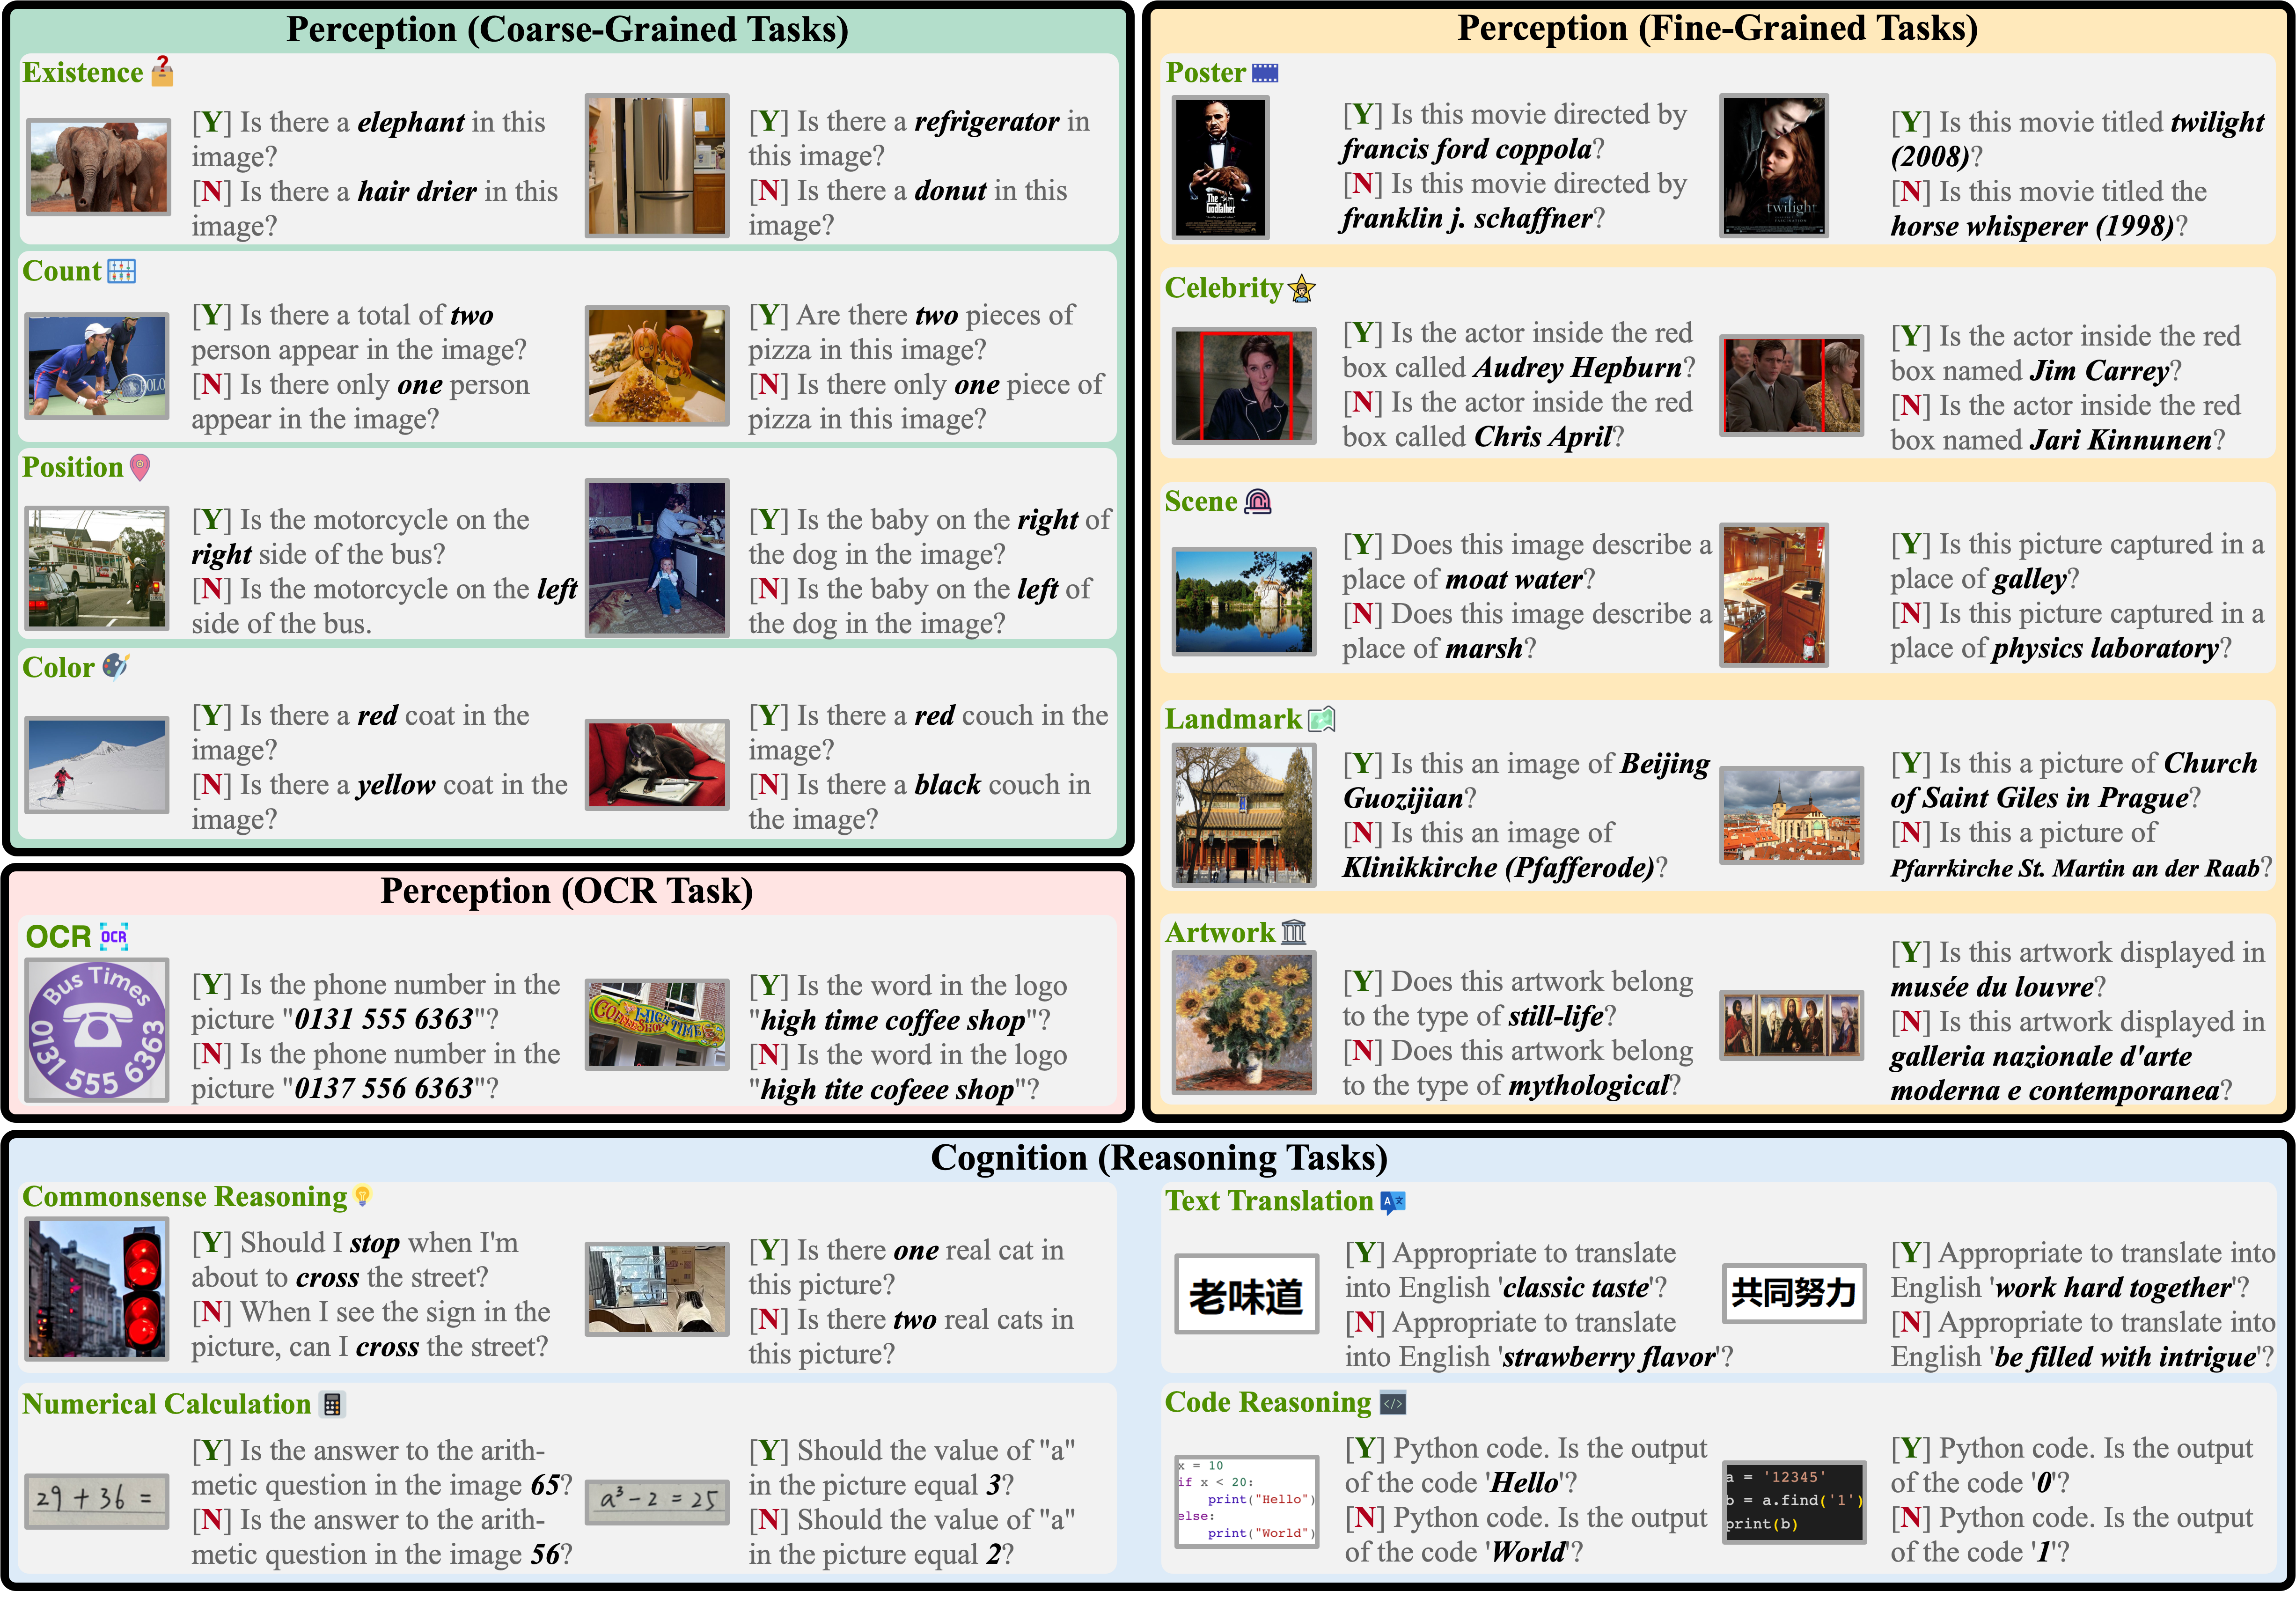
\includegraphics[width=.9\linewidth]{./p1.png}
\caption{\label{fig:org64412fd}Elo ratings of LLMs (Timeframe: April 24 - May 8, 2023) (\url{https://lmsys.org/blog/2023-05-10-leaderboard/})}
\end{figure}
\end{frame}

\begin{frame}[label={sec:org9cd988e}]{LLaMA: Open and Efficient Foundation Language Models \footfullcite{touvronLLaMAOpenEfficient2023}}
\begin{itemize}
\item The same model and architecture as GPT-2
\begin{itemize}
\item Replace ReLU with SwiGLU [PaLM] \footfullcite{shazeerGLUVariantsImprove2020}
\item Rotary Embeddings [GPTNeo] \footfullcite{suRoFormerEnhancedTransformer2022}
\end{itemize}
\item Publicly available datasets
\item 7B, 13B, 33B(30B?), 65B
\end{itemize}
\end{frame}

\begin{frame}[label={sec:orgd5893a6}]{LLaMA}
\begin{center}
\includegraphics[width=.9\linewidth]{./p2.png}
\end{center}
\end{frame}

\begin{frame}[label={sec:org6c7c162}]{Datasets}
\begin{center}
\includegraphics[width=.9\linewidth]{./p3.png}
\end{center}
\end{frame}

\begin{frame}[label={sec:orgb8281ab}]{Alpaca}
\begin{center}
\includegraphics[width=.9\linewidth]{./p4.jpg}
\end{center}
\end{frame}

\begin{frame}[label={sec:org5969e36},fragile]{Alpaca}
 \begin{minted}[]{json}
[{
    "instruction": "Rewrite the following sentence in the third person",
    "input": "I am anxious",
    "output": "She is anxious."
},
{
    "instruction": "What are the three primary colors?",
    "input": "",
    "output": "The three primary colors are red, blue, and yellow."
}]
\end{minted}
\end{frame}

\begin{frame}[label={sec:orgf626b32}]{Vicuna}
\begin{center}
\includegraphics[width=.9\linewidth]{./p5.png}
\end{center}
\end{frame}

\begin{frame}[label={sec:org25a3b38},fragile]{Vicuna}
 \begin{minted}[]{json}
[
  {
    "from": "human",
    "value": "Who are you?"
  },
  {
    "from": "gpt",
    "value": "My name is Vicuna, and I'm a language model developed by Large Model Systems Organization (LMSYS)."
  }
]
\end{minted}
\end{frame}

\begin{frame}[label={sec:orgc226713}]{Performance}
\begin{center}
\includegraphics[width=.9\linewidth]{./chart.png}
\end{center}
\end{frame}

\section{How?}
\label{sec:orgc9fa17d}

\begin{frame}[label={sec:orgaf9c15f}]{How?}
Follow Vicuna

\begin{itemize}
\item Dataset
\item LLaMA model parameters
\item Delta of Vicuna parameters (optional)
\item Fine-tuning
\end{itemize}
\end{frame}

\begin{frame}[label={sec:org496b6eb},fragile]{Datasets}
 \begin{minted}[]{json}
{
  "id": "identity_1",
  "conversations": [
    {
      "from": "human",
      "value": "Lab meeting on 5/12/2023"
    },
    {
      "from": "gpt",
      "value": "Recorder: yuzhi\n  Next week - Summary goals for summer\n  Consistent loss & Disagreement loss ..."
    }
  ]
}
\end{minted}
\end{frame}

\begin{frame}[label={sec:orga5b4558},fragile]{LLaMA and Vicuna model parameters}
 \begin{itemize}
\item Follow \url{https://huggingface.co/docs/transformers/main/model\_doc/llama}
\item \texttt{/data/public/LLaMA/download\_community.sh}
\begin{itemize}
\item run with \texttt{./download\_community.sh 7B /save/path}
\end{itemize}
\item \texttt{/data/public/LLaMA/*}
\end{itemize}
\end{frame}

\begin{frame}[label={sec:orgfb03ef6},fragile]{Fine-tuning}
 Follow: \url{https://github.com/lm-sys/FastChat}

Run with:

\begin{minted}[]{bash}
torchrun --nproc_per_node=4 --master_port=20001 fastchat/train/train_mem.py \
    --model_name_or_path ~/model_weights/llama-7b  \
    --data_path playground/data/dummy.json \
    --bf16 True \
    --output_dir output \
    --num_train_epochs 3 \
    --per_device_train_batch_size 2 \
    --per_device_eval_batch_size 2 \
    --gradient_accumulation_steps 16 \
    --evaluation_strategy "no" \
    --save_strategy "steps" \
    --save_steps 1200 \
    --save_total_limit 10 \
    --learning_rate 2e-5 \
    --weight_decay 0. \
    --warmup_ratio 0.03 \
    --lr_scheduler_type "cosine" \
    --logging_steps 1 \
    --fsdp "full_shard auto_wrap" \
    --fsdp_transformer_layer_cls_to_wrap 'LlamaDecoderLayer' \
    --tf32 True \
    --model_max_length 2048 \
    --gradient_checkpointing True \
    --lazy_preprocess True
\end{minted}
\end{frame}

\begin{frame}[label={sec:org58b8dc0},fragile]{Problem}
 \begin{itemize}
\item The size of tensor a (65537024) must match the size of tensor b (262148096)
\begin{itemize}
\item Need more data to fit batches
\end{itemize}
\item RuntimeError: CUDA out of memory
\begin{itemize}
\item change \texttt{python3.10/site-packages/torch/distributed/fsdp/\_state\_dict\_utils.py}
\item \texttt{state\_dict[fqn].clone().detach()} to \texttt{state\_dict[fqn].cpu().clone().detach()}
\end{itemize}
\end{itemize}
\end{frame}

\begin{frame}[label={sec:orga2c4bc0}]{Results}
\begin{description}
\item[{Ask}] Who is the Presenter on 4/14/2023 lab meeting?
\begin{itemize}
\item Playgroud data + Lab notes
\item Lab notes only
\end{itemize}
\end{description}

\begin{center}
\includegraphics[width=.9\linewidth]{./p6.png}
\end{center}
\end{frame}

\begin{frame}[label={sec:orgba4f7ad}]{Results}
\begin{itemize}
\item Playgroud data + Lab notes with 3 Epochs
\end{itemize}

\begin{center}
\includegraphics[width=.9\linewidth]{./p7.png}
\end{center}
\end{frame}

\begin{frame}[label={sec:orgd5c6734}]{Results}
\begin{itemize}
\item Playgroud data + Lab notes with 50 Epochs
\end{itemize}

\begin{center}
\includegraphics[width=.9\linewidth]{./p8.png}
\end{center}
\end{frame}

\begin{frame}[label={sec:org5a02397}]{Results}
\begin{itemize}
\item Lab notes with 3 Epochs
\end{itemize}

\begin{center}
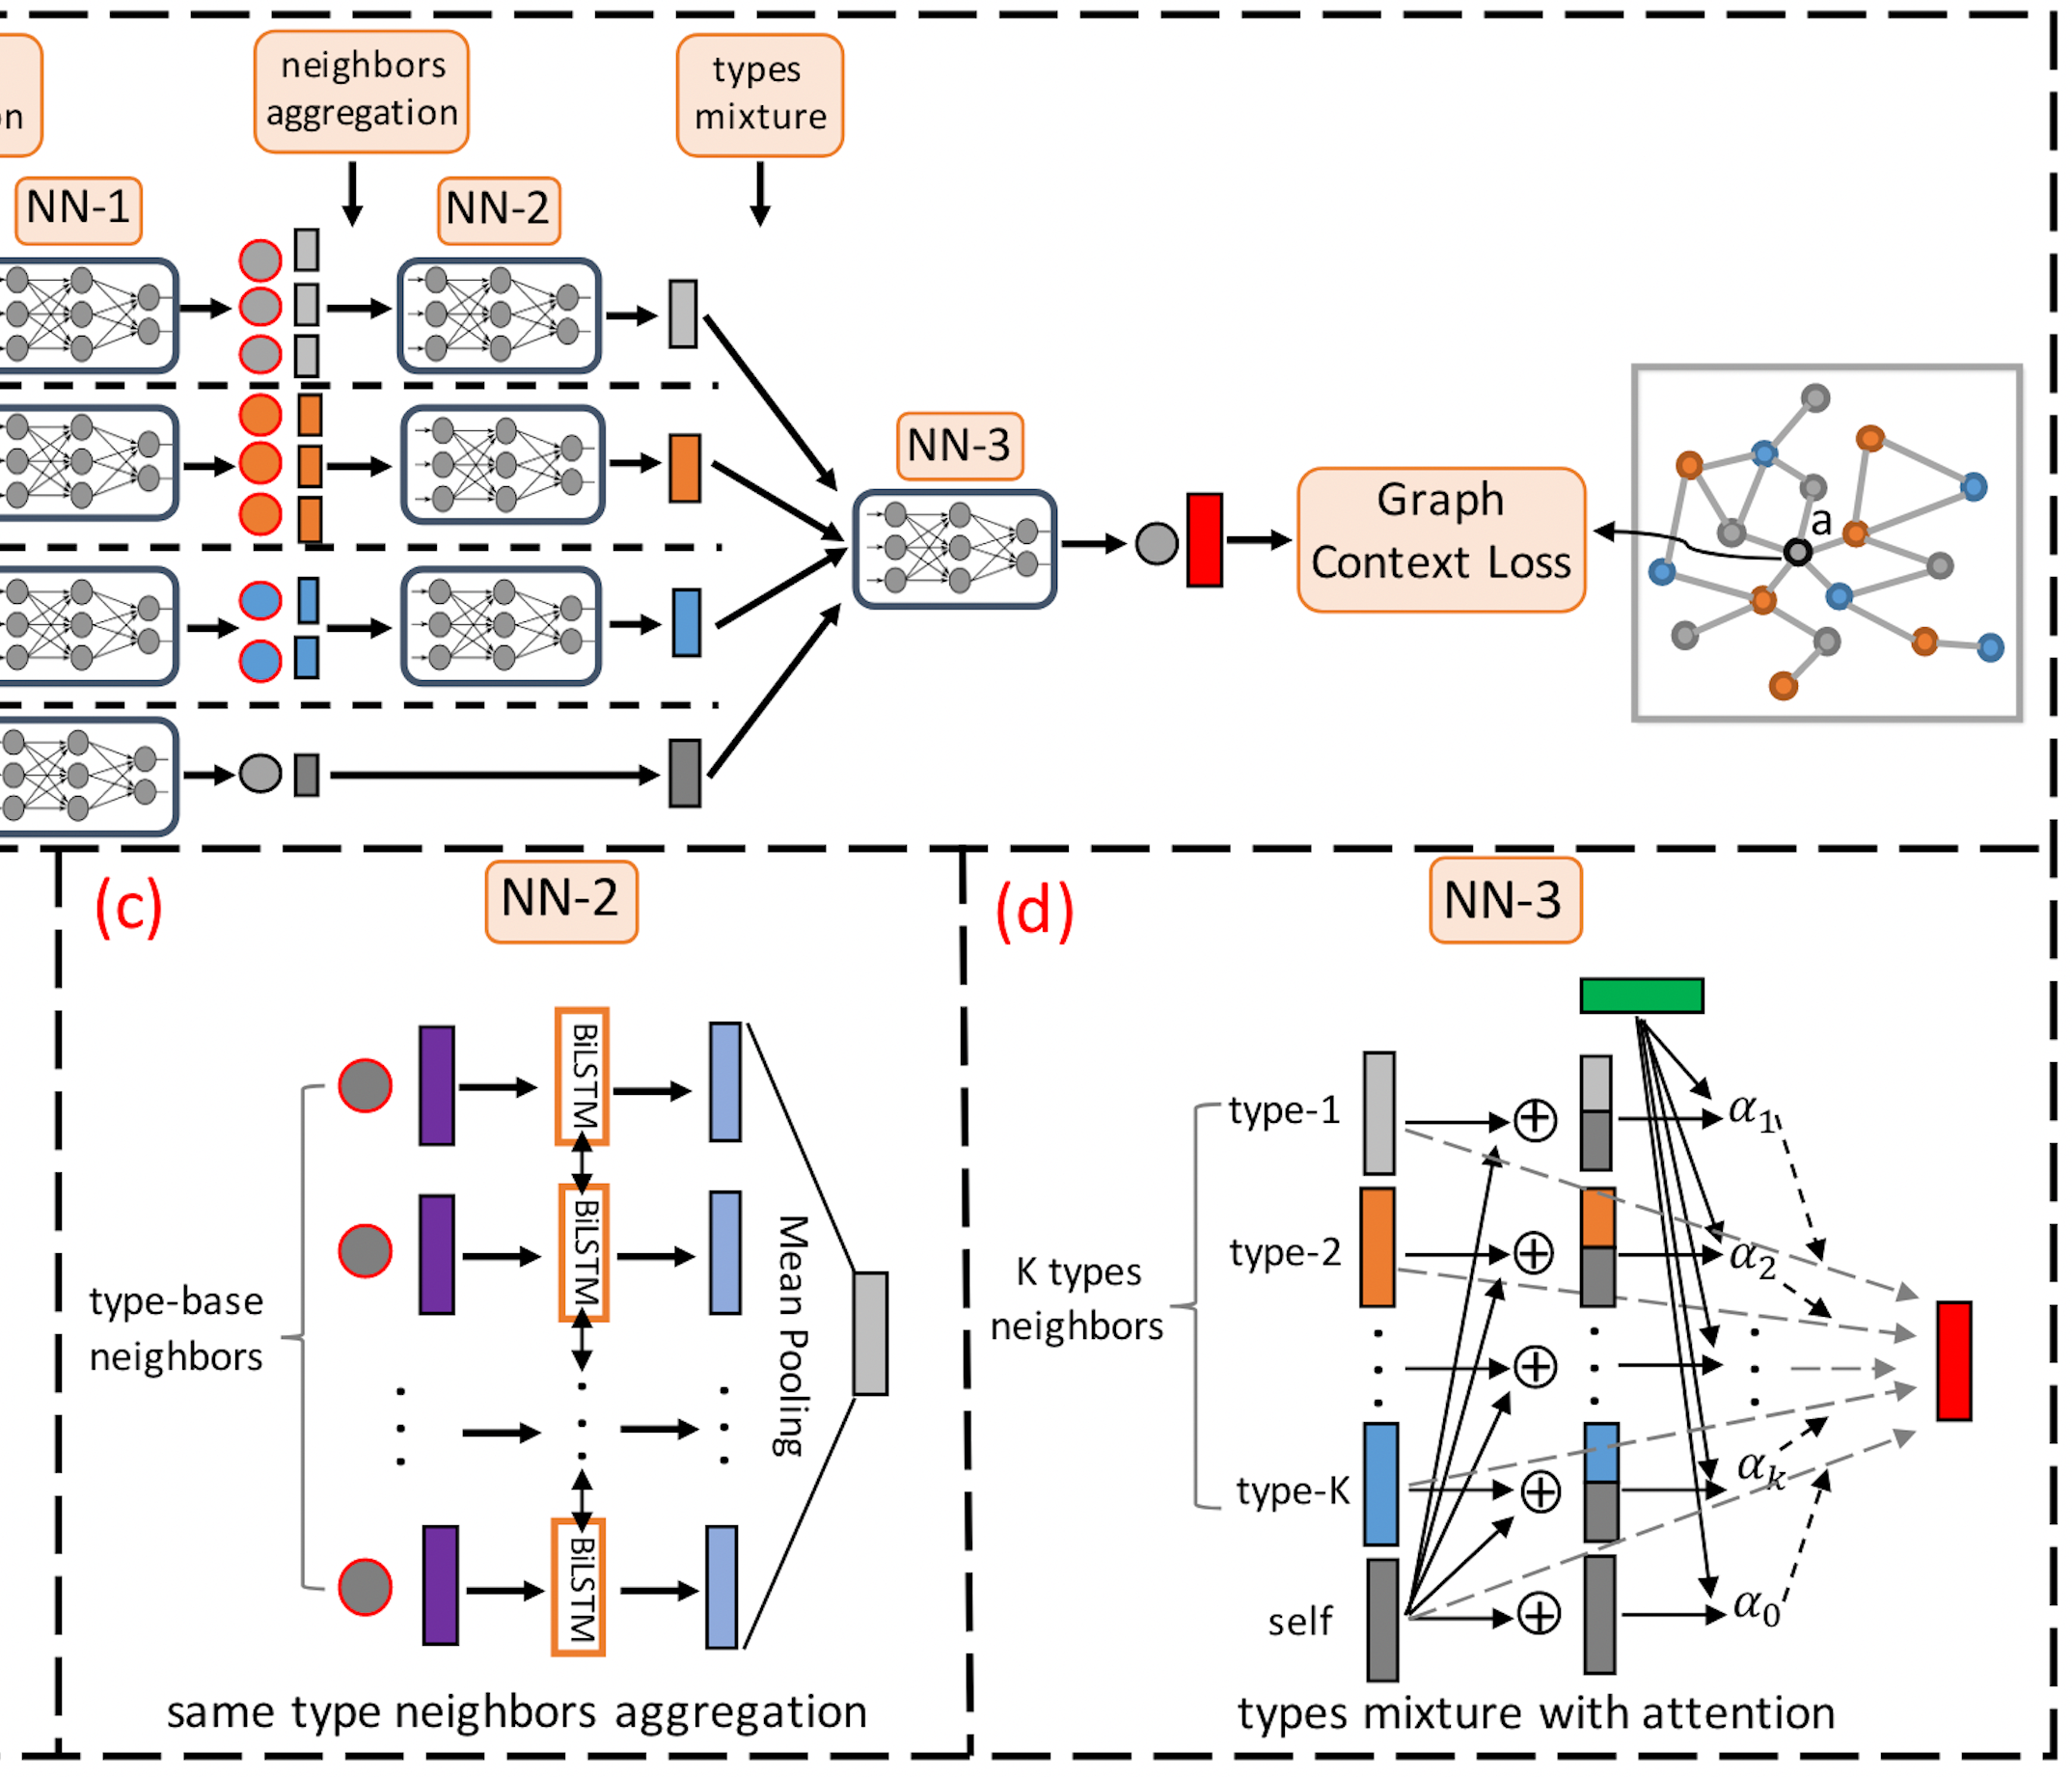
\includegraphics[width=.9\linewidth]{./p9.png}
\end{center}
\end{frame}

\begin{frame}[label={sec:org4bd3acc}]{Results}
\begin{itemize}
\item Lab notes with 50 Epochs
\end{itemize}

\begin{center}
\includegraphics[width=.9\linewidth]{./p10.png}
\end{center}
\end{frame}

\section{Conclusion}
\label{sec:org9410369}

\begin{frame}[label={sec:org29e2279}]{Conclusion}
\begin{itemize}
\item Which model to choice?
\begin{itemize}
\item From the rank \url{https://lmsys.org/blog/2023-05-10-leaderboard/}
\end{itemize}
\item How to fine-tune?
\begin{itemize}
\item Follow Vicuna FastChat framework
\item Follow Alpaca instruct framework
\end{itemize}
\end{itemize}
\end{frame}

\section{Reference}
\label{sec:orgcc95b53}

\begin{frame}[allowframebreaks]{Reference}
\printbibliography
\end{frame}

\section{Examples}
\label{sec:org9e588db}

\begin{frame}[label={sec:orgaf882d5}]{Example}
Outside.
\end{frame}
\end{document}